%----------------------------------------------------------------------------------------
%	PACKAGES AND THEMES
%----------------------------------------------------------------------------------------

\documentclass{beamer}

\mode<presentation> {

% The Beamer class comes with a number of default slide themes
% which change the colors and layouts of slides. Below this is a list
% of all the themes, uncomment each in turn to see what they look like.

%\usetheme{default}
%\usetheme{AnnArbor}
%\usetheme{Antibes}
%\usetheme{Bergen}
%\usetheme{Berkeley}
%\usetheme{Berlin}
%\usetheme{Boadilla}
%\usetheme{CambridgeUS}
%\usetheme{Copenhagen}
%\usetheme{Darmstadt}
%\usetheme{Dresden}
%\usetheme{Frankfurt}
%\usetheme{Goettingen}
%\usetheme{Hannover}
%\usetheme{Ilmenau}
%\usetheme{JuanLesPins}
%\usetheme{Luebeck}
\usetheme{Madrid}
%\usetheme{Malmoe}
%\usetheme{Marburg}
%\usetheme{Montpellier}
%\usetheme{PaloAlto}
%\usetheme{Pittsburgh}
%\usetheme{Rochester}
%\usetheme{Singapore}
%\usetheme{Szeged}
%\usetheme{Warsaw}

% As well as themes, the Beamer class has a number of color themes
% for any slide theme. Uncomment each of these in turn to see how it
% changes the colors of your current slide theme.

%\usecolortheme{albatross}
%\usecolortheme{beaver}
%\usecolortheme{beetle}
%\usecolortheme{crane}
%\usecolortheme{dolphin}
%\usecolortheme{dove}
%\usecolortheme{fly}
%\usecolortheme{lily}
%\usecolortheme{orchid}
%\usecolortheme{rose}
%\usecolortheme{seagull}
%\usecolortheme{seahorse}
%\usecolortheme{whale}
%\usecolortheme{wolverine}

%\setbeamertemplate{footline} % To remove the footer line in all slides uncomment this line
%\setbeamertemplate{footline}[page number] % To replace the footer line in all slides with a simple slide count uncomment this line

%\setbeamertemplate{navigation symbols}{} % To remove the navigation symbols from the bottom of all slides uncomment this line
}

\usepackage{graphicx} % Allows including images
\usepackage{booktabs} % Allows the use of \toprule, \midrule and \bottomrule in tables

\makeatletter
\setbeamertemplate{footline}
{
	\leavevmode%
	\hbox{%
		\begin{beamercolorbox}[wd=.333333\paperwidth,ht=2.25ex,dp=1ex,center]{author in head/foot}%
			\usebeamerfont{author in head/foot}\insertshorttitle %\insertauthor
		\end{beamercolorbox}%
		\begin{beamercolorbox}[wd=.333333\paperwidth,ht=2.25ex,dp=1ex,center]{title in head/foot}%
			\usebeamerfont{title in head/foot}\insertsection
		\end{beamercolorbox}%
		\begin{beamercolorbox}[wd=.333333\paperwidth,ht=2.25ex,dp=1ex,right]{date in head/foot}%
			\usebeamerfont{date in head/foot}\insertshortdate{}\hspace*{2em}
			\insertframenumber{} / \inserttotalframenumber\hspace*{2ex} 
		\end{beamercolorbox}}%
		\vskip0pt%
	}
\makeatother
	
%----------------------------------------------------------------------------------------
%	TITLE PAGE
%----------------------------------------------------------------------------------------

\title[HAShCache]{HAShCache : Heterogeneity Aware Shared DRAMCache
	for Integrated Heterogeneous Systems} % The short title appears at the bottom of every slide, the full title is only on the title page

\author{Adarsh Patil} % Your name
\institute[CSA, IISc] % Your institution as it will appear on the bottom of every slide, may be shorthand to save space
{
Department of Computer Science and Automation \\ Indian Institute of Science \\ % Your institution for the title page
\medskip
\textit{Advisor: Prof. R. Govindarajan} % Advisor
}
\date{\today} % Date, can be changed to a custom date

\begin{document}

\begin{frame}
\titlepage % Print the title page as the first slide
\centering \scriptsize{Submitted to 50th International Symposium on Microarchitecture (MICRO 2017)}
\end{frame}

\begin{frame}
\frametitle{Overview} % Table of contents slide, comment this block out to remove it
\tableofcontents % Throughout your presentation, if you choose to use \section{} and \subsection{} commands, these will automatically be printed on this slide as an overview of your presentation
\end{frame}

\note[itemize]{
	\item introduce IHS architecture, die stacking technology
	\item look at some motivation numbers for the work
	\item describe at the design decisions for hashcache and the heterogenity aware mechanisms of hashcache
	\item go over evalution methodology
	\item some results and the related work
}

%----------------------------------------------------------------------------------------
%	PRESENTATION SLIDES
%----------------------------------------------------------------------------------------

%------------------------------------------------
\section{Introduction}
%------------------------------------------------
\subsection{Intergrated Heterogenous Systems (IHS)} 

%------------------------------------------------
\begin{frame}
\frametitle{Introduction}
\begin{table}[]
\small
\centering
\begin{tabular}{@{}lll@{}}
	\toprule Criteria
	& \textbf{CPU}                                                                                     & \textbf{GPU}                                                                                  \\ \midrule
	\begin{tabular}[c]{@{}l@{}}number of \\ processing units\end{tabular} & 4-24 CPUs                                                                                        & 2048 processing units                                                                         \\ \midrule
	ILP                                                                   & 128 entry Re-order Buffer                                                                        & \begin{tabular}[c]{@{}l@{}}max 64 warps resident\\ (each warp has 32 threads)\end{tabular}    \\ \midrule
	\begin{tabular}[c]{@{}l@{}}Last Level SRAM\\ Cache\end{tabular}       & 1-4 MB                                                                                           & 700 KB - 1 MB                                                                                 \\ \midrule
	Memory                                                                & \begin{tabular}[c]{@{}l@{}}Large Main Memory\\ $\sim$ 10s - 100s GB\\ Allows Paging\end{tabular} & \begin{tabular}[c]{@{}l@{}}Limited Memory\\ $\sim$ 8 - 16 GB\\ No Paging support\end{tabular} \\ \midrule
	\begin{tabular}[c]{@{}l@{}}Programming\\ Paradigm\end{tabular}        & \begin{tabular}[c]{@{}l@{}}serial / multi-threaded /\\ SIMD\end{tabular}                         & SIMT, explicitly parallel                                                                     \\ \midrule
	Programming                                                           & Easy - Medium                                                                                    & Difficult                                                                                     \\ \midrule
	Power                                                                 & 1.5 GFLOPS/Watt                                                                                  & 5 GFLOPS / Watt                                                                               \\ \bottomrule
\end{tabular}
\label{cpu-vs-gpu}
\end{table}
\end{frame}

\note[itemize]{
	\item GPU have evolved from fixed function pipelines are being increasingly adopted for general purpose computing
	\item briefly look at some interesting arch characterisitics of CPU and GPU processors
	\item power 2012 K20 NVIDIA vs 2012 Sandybridge E5-2670
	\item energy efficiency of GPUs comes from simpler cores (small out of orders, no Branch pred)
	\item maybe add that GPU is streaming type of core
}
%------------------------------------------------

\begin{frame}
\frametitle{Integrated Heterogenous Systems (IHS) Architecture}
Latency-oriented CPU cores + Throughput-oriented GPGPU SMs \textbf{on-chip} \\
\begin{itemize}
	\item Simplifies Programming - Shared Virtual Memory, pointer sharing
	\item Allows GPGPUs to operate on data sets larger than memory size %using OS paging routines
	\item Reduces overall energy consumption
	\item Share resources - NoC, caches, memory controllers, DRAMs
	\item e.g. AMD APUs, Intel Iris, NVIDIA Denver
\end{itemize}
\begin{figure}[!htb]
	\centering
	\def\svgwidth{0.6\columnwidth}
	\input{arch.pdf_tex}
	%\caption{Architecture of an Integrated Heterogeneous System}
	\label{fig:hsa-arch}
\end{figure}
\end{frame}

\note[itemize]{
\item 99\% of Intel and 67\% of AMD non-server processors contain integrated graphics [APU 2013 summit]
\item most smartphones and tablet processors ship with heterogenous processors.
}
%------------------------------------------------
\subsection{3D Die-stacked DRAM} 

\begin{frame}
\frametitle{3D Die-stacked DRAM}
\begin{itemize}
\item DRAM layers placed closer to processing cores using 2.5D interposer and/or 3D TSV (through-silicon-vias)
\item Large capacity DRAM chips of the order of 100s of MBs to GBs
\item Large DRAM Bandwidth (beneficial for GPGPUs)
\item Better interconnect slightly lowers access latency (beneficial for CPUs)
\item Our proposal uses this capacity as a hardware managed cache
\item e.g. HBM (AMD/Hynix), HMC (Intel/Micron)
\end{itemize}
\begin{figure}[!htb]
	\centering
	\def\svgwidth{0.7\columnwidth}
	\input{stackedDRAM.pdf_tex}
	%\caption{Architecture of an Integrated Heterogeneous System}
	\label{fig:stacked-dram}
\end{figure}
\end{frame}

%------------------------------------------------
\section{Motivation}
%------------------------------------------------

\begin{frame}
\frametitle{Motivation}
(a) CPU Performance in IHS with Naive DRAMCache
    \begin{figure}
    	\includegraphics[scale=1]{graphs/motivation-cpu}
    \end{figure}
\begin{itemize}
\item CPU performance improves by 42\% over baseline IHS system without DRAMCache
\item Homogenous CPU archieves 372\% improvement with a DRAMCache
\item Performance gap of almost 260\%  compared to the ideal HoA CPU
\end{itemize} 
\end{frame} 
  
\begin{frame}
\frametitle{Motivation}    
(b) GPU Perfomance in IHS with Naive DRAMCache    
    \begin{figure}    	
    	\includegraphics[scale=1]{graphs/motivation-gpu}
    \end{figure}
\begin{itemize}
	\item GPU performance improves by 24\% over baseline IHS system with without DRAMCache
	\item Homogenous GPU archieves 35\% improvement with a DRAMCache
	\item Performance gap within 10\%  of its ideal HoA GPU
\end{itemize}    
\end{frame}

\begin{frame}
\frametitle{Motivation}
Cause for CPU Performance gap
	\begin{figure}
		\includegraphics[scale=1]{graphs/motivation-cpu-cache}
	\end{figure}
\begin{itemize}
	\item CPU Hit rates in DRAMCache marginally affected (about 4\%)
	\item Co-running with GPU increases the avg mem access latency by 213\%
\end{itemize}	
\end{frame}

%------------------------------------------------
\section{HAShCache Design}
%------------------------------------------------

\begin{frame}
\setbeamercovered{transparent}
	\frametitle{HAShCache Design}
\onslide<1->{
	\begin{block}{Metadata overhead}
		\small
		Caching at 128 byte granularity - Experimental results with 512 byte block under performs 128 bytes blocks by (12.2\%, 10.5\%) for (CPU,GPU)\\
		Tags stored in DRAM alongside data and streamed out in multiple bursts (TADs)
	\end{block}
}
\onslide<2->{
	\begin{block}{Set Associativity}
		\small
		Direct mapped cache organization
	\end{block}
}
\onslide<3->{
	\begin{block}{Reducing Miss Penalty}
		\small
		Cache Hit/miss Predictor based on MAP-I prediction for CPU \\
		No such mechanism for GPU
	\end{block}
}
\onslide<4->{
	\begin{block}{Addressing Scheme}
		\small
		Addressed with RBH addressing scheme (Row-Rank-Bank-Column-Channel) \\ 
		Experimental results show that BLP addressing scheme  (RoCoRaBaCh) performs worse by (3\%, 1\%) for (CPU,GPU)
	\end{block}	
}
\end{frame}

\note[itemize]{
	\item one needs to keep in mind several factors when designing a DRAM based cache as compared to a conventional cache
	\item several organizations have been proposed with various trade offs for DRAMCache in the cache parameters
	\item we re-examine these design decisions in the context of IHS architectures
}


%------------------------------------------------
\section{HAShCache Mechanisms}
%------------------------------------------------
\subsection{Heterogeneity aware DRAMCache scheduler - PrIS}


\begin{frame}
\frametitle{Heterogeneity aware DRAMCache scheduler - PrIS}
\emph{OBJECTIVE:} Reduce large access latencies for CPU req at DRAMCache
\begin{itemize}
	\onslide<2->{
	\item DRAM devices operate at lower clock rate and require periodic refresh which results in queueing of requests
	\item DRAM schedulers reorder requests to best suit DRAM characteristics (e.g. First Ready-FCFS)
	}
	\onslide<3->{
	\item In IHS processors,
	\begin{enumerate}
		\item large number of GPU requests $\implies$ exhaust the queue positions $\implies$ DRAMCache blocked and CPU requests being rejected
		\item GPU requests have good row buffer locality $\implies$ preferentially scheduled $\implies$ large queueing latency for CPU requests		
	\end{enumerate}
	}
\end{itemize}	
	\onslide<4->{
		
\begin{exampleblock}{CPU \underline{Pr}ioritized \underline{I}HS aware \underline{S}cheduler}
Queue entry reservation for CPU req  when queues reach critical levels\\
CPU Request Priorization when searching queues for next request to be serviced\\
Binary selection for scheduling simplifies the scheduling algorithm to a single stage and incurs no additional hardware overhead
	}
\end{exampleblock}	

\end{frame}

%------------------------------------------------

\subsection{Heterogeneity aware Temporal Bypass - ByE}
\begin{frame}
\frametitle{Heterogeneity aware Temporal Bypass - ByE}
\emph{OBJECTIVE:} Utilize the idle off-chip DRAM Bandwidth
	\only<1>{
\begin{itemize}		
	\item Large DRAMCache capacity $\implies$ high hit rates and long block residency time before being evicted $\implies$ under-utilized off-chip DRAM bandwidth
	\item Baseline incorporates a hit/miss predictor for CPU requests and starts early off-chip access for a request that is predicted to be a miss	
	
	\hspace{5em}
	\def\svgwidth{0.5\linewidth}
	\input{before-bye.pdf_tex}
	
	\item However, we observe that when GPU is running, CPU requests returning from off-chip access wait at DRAMCache for verification of hit/miss via a tag match
\end{itemize}
	}
	
	\only<2>{
		
\begin{exampleblock}{\underline{By}pass \underline{E}nabler (ByE)}
Bypasses CPU requests to clean lines and cache misses when the GPU is running \\
Achieved using a Counting Bloom Filter that tracks dirty lines in the DRAMCache \\
\end{exampleblock}
	
	\hspace{5em}
	\def\svgwidth{0.5\linewidth}
	\input{bye.pdf_tex}
\begin{itemize}		
	\item Bypassed CPU requests are not filled into DRAMCache
	\item Hardware Overhead: 256KB (0.4\% of cache capacity)
\end{itemize}	
	}
\end{frame}

\note[itemize]{
	\item not filling CPU responses into D\$ allows to maintain bypass efficiency and reduce bandwidth bloat due to miss fill
}
%------------------------------------------------

\subsection{Heterogeneity aware Spatial Occupancy Control - Chaining}
\begin{frame}
\frametitle{Heterogeneity aware Spatial Occupancy Control - Chaining}
\emph{OBJECTIVE:} Allow GPU to better use DRAMCache Bandwidth
Observations: 
\begin{itemize}
	\item GPU Hit rates in DRAMCache should be high enough that the GPU requests donot have to frequently use the relatively constricted off-chip DRAM bus
	\item GPU can trade off access latency for higher hit rates
	\item CPU applications have smaller working sets of a few MBs
	\item Small size GPU L2 caches provide limited filtering of traffic as compared to the CPU L2 cache
\end{itemize}
\begin{exampleblock}{Chaining}
Introduces pseudo associativity for GPU \\
Ensures minimum occupancy of CPU lines in the DRAMCache
\end{exampleblock}

\end{frame}

%------------------------------------------------
\begin{frame}
\frametitle{Heterogeneity aware Spatial Occupancy Control - Chaining}
\begin{columns}[c]
	
\column{0.7\linewidth}
\begin{itemize}
	\item Linear probing like scheme to resolve conflicts
	\item Maintains low-threshold value ($l_{cpu}$) occupancy for CPU lines in DRAMCache by ensuring GPU line does not replace CPU lines when this threshold is reached
	\item For a GPU line evicting a GPU line, chaining tries to replace a CPU line in any of the consecutive 3 locations
	\item For all CPU requests, data is always inserted into the original location
	\item Chained set location is represented by a 2 bit offset (used for lookup) + 2 bit reverse chain bits for the chained set (used for eviction)
	\item psuedo-associativity of atmost 1 and atmost 2 tag matches are needed
\end{itemize}

\column{0.3\linewidth}

\def\svgwidth{\linewidth}
\input{chainings.pdf_tex}

\end{columns}
\end{frame}

\note[itemize]{
	\item define original set and chained set
	\item psuedo assoc of atmost 1
}
%------------------------------------------------
\begin{frame}
\frametitle{Heterogeneity aware Spatial Occupancy Control - Chaining}
\begin{figure}
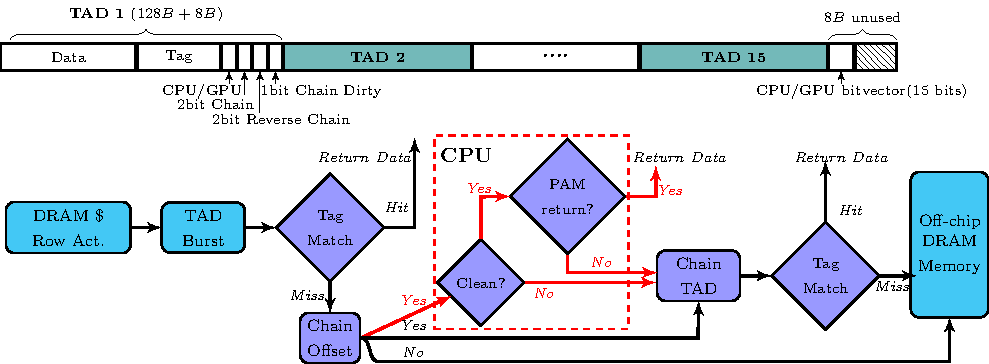
\includegraphics[scale=0.7]{chaining}
\end{figure}
Chaining organization within the DRAMCache row and working
\begin{itemize}
	\item CPU/GPU share address space, hence require both sets to be checked
	\item Chain dirty bits avoid second set lookup for CPU
	\item Chain offset, Reverse chain offset, Chain dirty bits, set ownership information uses the unused bits in the DRAMCache row
\end{itemize}
\end{frame}

\note[itemize]{
	\item no hardware overhead incurred
}
%------------------------------------------------
\section{Evaluation Methodology}
\begin{frame}
	\frametitle{Experimental Setup}
\begin{columns}[c]
\column{.75\textwidth}
	
	\begin{table}[h]
		\footnotesize
		\centering
		\begin{tabular}{{@{}ll@{}}}
			\toprule
			CPU Core 	& five 4-wide OoO x86 cores @2.5 GHz \\
			\midrule
			CPU Caches 	& 32KB 8-way split I/D private L1 Cache, \\ 
			& 1MB 8-way shared split L2 Cache, 128B lines \\
			\midrule
			GPU Core 	& eight Fermi SMs@700MHz, 2x2 GTO warp sched\\
			& 64K registers, 96KB scratch memory \\
			\midrule
			GPU Caches 	& 64KB 4-way private L1 cache,\\ 
			& 512KB, 16-way assoc L2 Coherent Cache \\
			\midrule
			Stacked     & 2 vaults, HMC\_2500\_x64, 2KB Page \\
			DRAM		& $t_{CL}$-$t_{RCD}$-$t_{RP}$-$t_{RAS}$=9.9ns-10.2ns-7.7ns-21.6ns\\
			& 8 layers/vault, 4 banks/layer\\
			& 64 byte burst size, Peak bandwidth 40GB/s \\
			%& Refresh related: $t_{REFI}$=3.9us $t_{RFC}$=59us \\
			\midrule
			Off-chip 	& 2 channels, DDR3\_1600\_x64, 1KB page \\
			DRAM		& $t_{CL}$-$t_{RCD}$-$t_{RP}$-$t_{RAS}$=13.75ns-13.75ns-13.75ns-35ns\\
			& 1 rank/channel, 8 banks/rank\\
			& 64 byte burst size, Peak bandwidth 25GB/s \\
			%& Refresh related: $t_{REFI}$=7.8us $t_{RFC}$=260us \\
			\bottomrule
		\end{tabular}
		\caption{Configuration of the simulated system}
		\label{configuration}
	\end{table}
		
	\column{.3\textwidth}
	\footnotesize
	\textbf{Simulator}
	\begin{itemize}
		\item gem5-gpu
		\item SE mode
		\item Heterogenous Cache Coherence
	\end{itemize}
	\textbf{DRAMCache}
	\begin{itemize}
		\item Memory-side cache 
		%\item HMC-like
		\item MSHR, WriteBuffers
		\item Fill Queue
		\item Non-inclusive
	\end{itemize}
	
\end{columns}
\end{frame}

%------------------------------------------------

\begin{frame}
\frametitle{Methodology}
    Medium to high memory intensive \emph{Multi-programmed SPEC 2006} combinations on CPU coupled with a \emph{Rodinia no-copy} GPU benchmark
	\begin{table}[h!]
		\footnotesize
		\centering
		\begin{tabular}{{|l|l|l|}}
			\hline
			\textbf{Name} & \textbf{Multi-program SPEC2006} & \textbf{Rodinia}\\
			\hline
			Qg1& cactusADM;gcc;bzip2;sphinx3 & needle\\
			\hline
			Qg2 & astar;mcf;gcc;bzip2 & needle\\
			\hline
			Qg3 & gcc;libquantum;leslie3d;bwaves & needle\\
			\hline
			Qg4 & astar;soplex;cactusADM;libquantum & k-means\\
			\hline
			Qg5 & milc;mcf;libquantum;bzip2 & k-means\\
			\hline
			Qg6 & bzip2;gobmk;hmmer;sphinx3 & k-means\\
			\hline
			Qg7 & soplex;milc;cactusADM;libquantum & gaussian\\
			\hline
			Qg8 & milc;libquantum;gobmk;leslie3d & gaussian\\
			\hline
			Qg9 & astar;milc;gcc;leslie3d & hotspot\\
			\hline
			Qg10 & gcc;gobmk;leslie3d;sphinx3 & hotspot\\
			\hline
			Qg11 & astar;cactusADM;libquantum;sphinx3 & srad\\
			\hline
			Qg12 & astar;mcf;gobmk;sphinx3 & streamcluster\\
			\hline
			Qg13 & astar;cactusADM;libquantum;sphinx3 & lud\\
			\hline
		\end{tabular}
		\caption{Workloads}
		\label{workloads}
	\end{table}
\end{frame}

%------------------------------------------------
\begin{frame}
\frametitle{Methodology}
\begin{itemize}
	\item Fast-forward init phase until just before launch of the first kernel of the GPU program
	\item Each CPU forwarded by atleast 2B instructions (avg 20B per mix)
	\item Warmup phase until the fastest core reaches 250M instructions
	\item Detailed Timing simulations - atleast 250M instructions on each core
	\item Rodinia benchmarks run in a \textit{conditioned loop} represents the ROI
	\item CPU performance considered for first 250M instructions
	\item GPU performance considered for the first execution of the \textit{conditioned loop} or the last completed kernel whichever is earlier
	\item Performance Metric - Harmonic mean, Weighted Speedup
	{\scriptsize
		\begin{equation*}
		H\textnormal{-}MEAN_{CPU} = \frac{n_{cpu}}{\sum_{i=1}^{n_{cpu}} \frac{1}{IPC_{i}^{CPU}}}, \hspace{0.2cm} H\textnormal{-}MEAN_{GPU} = \frac{n_{gpu}}{\sum_{i=1}^{n_{gpu}} \frac{1}{IPC_{i}^{GPU}}} 
		\end{equation*}
	}
	{\scriptsize
		\begin{equation*}
		H\textnormal{-}MEAN_{IHS} = \frac{n_{cpu}+ n_{gpu}}{\sum_{i=1}^{n_{cpu}} \frac{1}{IPC_{i}^{CPU}} + \sum_{i=1}^{n_{gpu}} \frac{1}{IPC_{i}^{GPU}}}, 
		WS = \sum_{i=1}^{n_{cpu}} \frac{IPC_i^{CPU_{IHS}}}{IPC_i^{SP}} + \sum_{i=1}^{n_{gpu}} \frac{IPC_i^{GPU_{IHS}}}{IPC_i^{GPU}}
		\end{equation*}
	}
\end{itemize}
\end{frame}

%------------------------------------------------

%------------------------------------------------
\section{Results}
%------------------------------------------------

\begin{frame}
\frametitle{Results - Individual CPU and GPU performance}
\begin{figure}
\includegraphics[width=\linewidth]{graphs/results-cpu}
\end{figure}
\begin{figure}
\includegraphics[width=\linewidth]{graphs/results-gpu}
\end{figure}
\end{frame}

%------------------------------------------------

\begin{frame}
	\frametitle{Results - System Performance}
	\begin{figure}
		\includegraphics[width=\linewidth]{graphs/results-system}
	\end{figure}
	\begin{figure}
		\includegraphics[width=\linewidth]{graphs/results-weighted-speedup}
	\end{figure}
\end{frame}

%------------------------------------------------

\begin{frame}
\frametitle{Sensitivity Study with 128MB DRAMCache}
\begin{figure}
\includegraphics[width=0.9\linewidth]{graphs/results-128M-cpu}
\end{figure}
\begin{figure}
	\includegraphics[width=0.9\linewidth]{graphs/results-128M-gpu}
\end{figure}
\end{frame}


%------------------------------------------------
\section{Conclusion, Related Work}
%------------------------------------------------

\begin{frame}[fragile] % Need to use the fragile option when verbatim is used in the slide
\frametitle{Conclusion}
\begin{itemize}
	\item We present a case for performance improvement of IHS with a stacked DRAMCache device
	\item Quantify the effects of co-running on each processor and show that heterogeneity adversely affects CPU performance 
	\item We carefully design a DRAMCache organization for IHS processors
	\item We propose 3 heterogeniety-aware optimizations for DRAMCache - a scheduler, a spatial bypass and a temporal occupancy control scheme that improves performance of the overall system by over 200\% over a systen with no DRAMCache and 41\% over a system with a naive DRAMCache
	\item Significant benefits of using a stacked DRAMCache for IHS processors, far exceeding the usefulness of the such devices in homogeneous GPUs and multi-core CPU systems.
\end{itemize}
\end{frame}

%------------------------------------------------

\begin{frame}
\frametitle{Related Work and References}
\scriptsize{
\begin{thebibliography}{99} % Beamer does not support BibTeX so references must be inserted manually as below
\bibitem[alloycache]{p1} M. K. Qureshi and G. H. Loh
\newblock Fundamental latency trade-off in architecting dram caches: Outperforming impractical sram-tags with a simple and practical design
\newblock \emph{MICRO-45, 2012}


\bibitem[sms]{p2} R. Ausavarungnirun, K.K.W. Chang, L. Subramanian, G. H. Loh, and O. Mutlu
\newblock Staged memory scheduling: Achieving high performance and scalability in heterogeneous systems
\newblock \emph{ISCA-39, 2012}

\bibitem[warp]{p4} O. Kayiran, N. C. Nachiappan, A. Jog, R. Ausavarungnirun, M. T. Kandemir, G. H. Loh, O. Mutlu, and C. R. Das
\newblock Managing gpu concurrency in heterogeneous architectures
\newblock \emph{MICRO-47, 2014}

\bibitem[oscar]{p3} J. Zhan, O. Kayiran, G. H. Loh, C. R. Das, and Y. Xie
\newblock Oscar: Orchestrating stt-ram cache traffic for heterogeneous cpu-gpu architectures
\newblock \emph{MICRO-49, 2016}

\bibitem[tap]{p4} J. Lee and H. Kim
\newblock Tap: A tlp-aware cache management policy for a cpu-gpu heterogeneous architecture
\newblock \emph{HPCA-18, 2012}

\bibitem[helm]{p4} V. Mekkat, A. Holey, P.C. Yew, and A. Zhai
\newblock Managing shared last-level cache in a heterogeneous multicore processor
\newblock \emph{PACT-22, 2013}

\end{thebibliography}
}
\end{frame}

%------------------------------------------------

\begin{frame}
\frametitle{Thank You}
\Huge{\centerline{Questions? }}
\end{frame}

%----------------------------------------------------------------------------------------

\end{document}